% Provenance (never printed): see sources/outline_sources.md (Year 3: gravitational
% potential, spherical harmonics, J2, reference ellipsoid, geoid, satellite gravimetry,
% flexure of the lithosphere). Brief: sources/book5/BRIEFS.md, ch. 3. Curves from
% figdata/bachelor-3/hydrostatic_figure.py, ice_mass.py (IMBIE 2021), flexure.py.
% Exercise and problem values in the Book 5 scratch calculator calc/ch03.py.
\chapter{Gravidade e a figura da Terra}\label{ch:b3:gravity-geodesy}

Dois satélites voam um atrás do outro em torno da Terra, a uma altitude de mais de
\qty{500}{km} e separados por cerca de \qty{220}{km}, e medem a distância entre
eles o tempo todo, com precisão de um micrômetro.
% ledger: geod5:grace, geod5:grace-ranging
Quando passam sobre um lugar com massa concentrada, o satélite da frente é
puxado primeiro e a distância aumenta; em seguida, o de trás é puxado e a
distância diminui. A partir dessas variações minúsculas, mês a mês desde 2002, o
campo gravitacional da Terra vem sendo mapeado em sua mudança: a água armazenada
nas bacias dos rios sobe e desce com as estações, e os grandes mantos de gelo da
Groenlândia e da Antártida perdem massa ano após ano. A gravidade pesa o que o
olho não consegue ver. Este capítulo constrói o campo gravitacional de um planeta em rotação a partir de seu
potencial, obtém nele o achatamento e o momento de inércia, acompanha suas
anomalias até a órbita e, então, volta-se para uma das coisas que a gravidade revela na
superfície: a flexão da litosfera sob o peso de um vulcão.

\begin{recall}
A lei da gravitação de Newton, a energia potencial gravitacional e a força
centrífuga em um referencial girante são assunto dos livros de física; os momentos
de inércia de um sólido e os polinômios de Legendre $P_2(x) = (3x^2 - 1)/2$ estão
nos volumes universitários de física e de matemática, o módulo de Young $E$ e o
coeficiente de Poisson $\nu$ no volume do terceiro ano dos livros de física. Geodésia e o achatamento $f = (a - b)/a$ de um elipsoide de semieixos $a > b$
foram vistos no 10º ano. Isostasia, compensação de Airy,
gravidade normal, geoide, altura do geoide e anomalias da gravidade foram
definidas no volume do primeiro ano, em seu capítulo sobre isostasia e anomalias
da gravidade.
\end{recall}

\section{O geopotencial}

Em um planeta em rotação, um corpo em repouso sente a atração da massa do planeta
e, no referencial que gira com ele, a força centrífuga. Ambas derivam de um
potencial.

\begin{definition}[Geopotencial]\label{def:b3:gravity-geodesy:geopotential}
O \emph{geopotencial}\index{geopotencial} é a energia potencial por unidade de
massa, no referencial girante com a Terra à velocidade angular $\omega$, da
gravitação e da força centrífuga em conjunto:
\[
  W(\mathbf r) = V(\mathbf r) + \Phi(\mathbf r),\qquad
  V(\mathbf r) = -G\int_{\text{Terra}}\frac{\mathrm dm'}{|\mathbf r - \mathbf r'|},\qquad
  \Phi(\mathbf r) = -\tfrac12\omega^2 s^2,
\]
Em que $s$ é a distância ao eixo de rotação. A gravidade é
$\mathbf g = -\nabla W$, e as superfícies $W = \text{const}$ são suas superfícies
equipotenciais: a gravidade é, em toda parte, normal a elas.
\end{definition}

Um fio de prumo se alinha com $-\nabla W$, e a água parada assenta sobre uma
superfície equipotencial. Um planeta fluido em rotação, portanto, assume a forma
de uma de suas próprias superfícies equipotenciais: o potencial centrífugo, mais
profundo no equador, incha o equador e achata os polos.

\begin{omfigure}
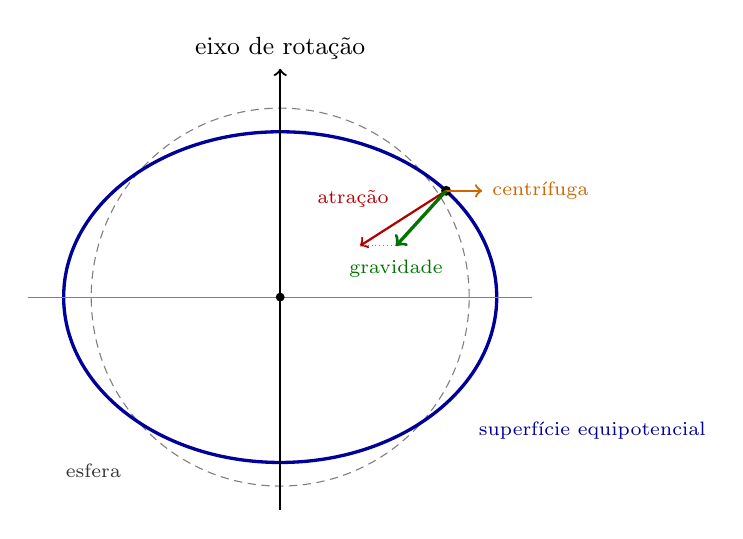
\begin{tikzpicture}[font=\small, x=1cm, y=1cm]
\draw[gray, densely dashed] (0,0) circle (2.4);
\draw[very thick, blue!60!black] (0,0) ellipse (2.75 and 2.1);
\draw[->, thick] (0,-2.7) -- (0,2.9) node[above] {eixo de rotação};
\draw[gray] (-3.2,0) -- (3.2,0);
\fill (0,0) circle (1.6pt);
% a point at latitude 40 deg (parameter) on the ellipse; the attraction points at
% the centre, the centrifugal force is horizontal, and their sum is drawn along the
% inward normal of the ellipse: lengths solved so that the sum is normal (calc/ch03_fig.py)
\coordinate (P) at (2.107,1.350);
\fill (P) circle (1.8pt);
\draw[->, thick, red!70!black] (P) -- (1.012,0.650);
\node[font=\scriptsize, red!70!black, anchor=south east] at (1.50,1.02) {atração};
\draw[->, thick, orange!80!black] (P) -- (2.565,1.350) node[right, font=\scriptsize] {centrífuga};
\draw[gray, densely dotted] (1.012,0.650) -- (1.470,0.650);
\draw[->, very thick, green!45!black] (P) -- (1.470,0.650);
\node[font=\scriptsize, green!45!black, anchor=north] at (1.470,0.600) {gravidade};
\node[blue!60!black, anchor=west, font=\scriptsize] at (2.4,-1.7) {superfície equipotencial};
\node[gray!40!black, anchor=east, font=\scriptsize] at (-1.9,-2.2) {esfera};
\end{tikzpicture}

\par\smallskip{\small Uma superfície equipotencial de um planeta em rotação (esquemática,
com o achatamento muito exagerado). Em cada ponto, a gravidade, soma da atração e
da força centrífuga, é normal à superfície equipotencial; ela não aponta para o
centro, exceto nos polos e no equador.}
\label{fig:b3:gravity-geodesy:equipotential}
\end{omfigure}

Fora do planeta, o potencial gravitacional obedece à equação de Laplace, e
suas soluções regulares no infinito são os harmônicos esféricos sólidos.

\begin{proposition}[Expansão em harmônicos esféricos do geopotencial]\label{prop:b3:gravity-geodesy:harmonics}
Fora de um corpo de massa $M$ e raio equatorial $a$, com a origem em seu centro de
massa e o eixo $z$ ao longo de seu eixo de rotação, o potencial gravitacional à
distância $r$, colatitude $\theta$ e longitude $\lambda$ é
\begin{multline*}
  V = -\frac{GM}{r}\Biggl[1 - \sum_{n=2}^{\infty}\left(\frac ar\right)^nJ_nP_n(\cos\theta)\\
  + \sum_{n=2}^{\infty}\sum_{m=1}^{n}\left(\frac ar\right)^nP_{nm}(\cos\theta)
  (C_{nm}\cos m\lambda + S_{nm}\sin m\lambda)\Biggr],
\end{multline*}
com os polinômios de Legendre $P_n$ e as funções associadas $P_{nm}$; os coeficientes
$J_n$, $C_{nm}$, $S_{nm}$ são números, ajustados a observações. Para um corpo
simétrico em torno de seu eixo, restam apenas os termos zonais $J_n$. Não aparece
nenhum termo de grau 1.
\end{proposition}

\begin{proof}
A separação de variáveis da equação de Laplace em coordenadas esféricas
fornece as soluções regulares no infinito $r^{-(n+1)}P_{nm}(\cos\theta)e^{\pm
im\lambda}$ (os volumes universitários de matemática); qualquer potencial fora das
massas é uma soma delas. O termo de grau 0 é $-GM/r$, o potencial da massa
inteira. Os termos de grau 1 são proporcionais aos primeiros momentos
$\int\mathbf r'\,\mathrm dm'$, que se anulam quando a origem está no centro de
massa. A simetria axial elimina todo termo que depende de $\lambda$.
\end{proof}

\begin{definition}[Fator de forma dinâmico]\label{def:b3:gravity-geodesy:j2}
O \emph{fator de forma dinâmico}\index{fator de forma dinâmico} $J_2$ de um planeta
é o coeficiente de seu harmônico zonal de grau 2: o maior desvio de seu
potencial externo em relação ao de uma esfera, causado por seu achatamento. Para a
Terra, $J_2 = \num{1.08263e-3}$.
% ledger: geod5:grs80-defining
\end{definition}

\begin{theorem}[Fórmula de MacCullagh]\label{thm:b3:gravity-geodesy:maccullagh}
Sejam $A$, $B$, $C$ os momentos principais de inércia de um corpo de massa $M$
em torno de eixos que passam por seu centro de massa, e $I$ seu momento de inércia
em relação à reta que vai do centro de massa a um ponto externo à distância $r$. Até
a ordem $r^{-3}$, o potencial gravitacional nesse ponto é dado pela
\emph{fórmula de MacCullagh}\index{fórmula de MacCullagh}
\[
  V = -\frac{GM}{r} - \frac{G(A + B + C - 3I)}{2r^3} .
\]
Para um corpo simétrico em relação ao eixo $z$ ($A = B$),
$V = -\dfrac{GM}{r} + \dfrac{G(C - A)}{r^3}P_2(\cos\theta)$, de modo que
\[
  J_2 = \frac{C - A}{Ma^2} .
\]
\end{theorem}

\begin{proof}
Com $\hat{\mathbf r}$ o vetor unitário apontando para o ponto e $r' \ll r$,
\[
  \frac{1}{|\mathbf r - \mathbf r'|} = \frac1r + \frac{\hat{\mathbf r}\cdot\mathbf r'}{r^2}
  + \frac{3(\hat{\mathbf r}\cdot\mathbf r')^2 - r'^2}{2r^3} + O(r^{-4}).
\]
Integrando sobre a massa, o primeiro termo dá $M/r$ e o segundo se anula
(centro de massa). Para o terceiro, $\int r'^2\,\mathrm dm' = (A + B + C)/2$, pois
$A + B + C = \int 2r'^2\,\mathrm dm'$, e $\int(\hat{\mathbf r}\cdot\mathbf
r')^2\,\mathrm dm' = \int r'^2\,\mathrm dm' - I$, já que o quadrado da distância à
reta é $r'^2 - (\hat{\mathbf r}\cdot\mathbf r')^2$. O colchete integra-se
a $3(A + B + C)/2 - 3I - (A + B + C)/2 = A + B + C - 3I$. Para $A = B$, o
momento em relação a uma reta de colatitude $\theta$ é $I = A\sin^2\theta + C\cos^2\theta$,
e $2A + C - 3I = (C - A)(1 - 3\cos^2\theta) = -2(C - A)P_2(\cos\theta)$.
Comparando com a \cref{prop:b3:gravity-geodesy:harmonics} resulta
$J_2Ma^2 = C - A$.
\end{proof}

O termo de grau 2 do potencial, portanto, mede a diferença dos
momentos de inércia, e não os próprios momentos. A precessão do eixo da Terra,
provocada pelos torques do Sol e da Lua sobre o abaulamento equatorial,
mede a elipticidade dinâmica $H = (C - A)/C$; juntos, $J_2$ e $H$ fornecem
$C/(Ma^2)$, o fator de momento de inércia, \num{0.3308} para a Terra,
% ledger: earth:MoI
bem abaixo dos \num{0.4} de uma esfera uniforme: a massa está concentrada em direção
ao centro.

\section{O elipsoide girante}

\begin{definition}[Elipsoide de referência]\label{def:b3:gravity-geodesy:ellipsoid}
Um \emph{elipsoide de referência}\index{elipsoide de referência} é um elipsoide de
revolução, de semieixo equatorial $a$ e achatamento $f$, escolhido de modo que seja
ele próprio uma superfície de nível de um potencial modelo: o potencial de um corpo
girante de massa $M$ com velocidade angular $\omega$ e o \omterm{def:b3:gravity-geodesy:j2}{fator de forma dinâmico}
$J_2$ da Terra. Quatro constantes o definem; o Sistema de Referência Geodésico de
1980 adota
\begin{gather*}
  a = \qty{6378137}{m},\qquad GM = \qty{3.986005e14}{m^3.s^{-2}},\\
  J_2 = \num{1.08263e-3},\qquad \omega = \qty{7.292115e-5}{rad.s^{-1}},
\end{gather*}
e deduz deles o achatamento $f = \num{0.00335281068}$
($1/f = \num{298.257222}$) e o semieixo menor
$b = \qty{6356752.3141}{m}$.
% ledger: geod5:grs80-defining, geod5:grs80-derived
\end{definition}

O potencial do modelo, o potencial normal, é conhecido em forma fechada, e também
sua gravidade sobre o elipsoide, a gravidade normal do volume do primeiro ano.

\begin{proposition}[Fórmula de Somigliana]\label{prop:b3:gravity-geodesy:somigliana}
Em um \omterm{def:b3:gravity-geodesy:ellipsoid}{elipsoide de referência} com semieixos $a$, $b$ e gravidade normal
$\gamma_e$ no equador e $\gamma_p$ nos polos, a gravidade normal na latitude
geodésica $\varphi$ é dada pela \emph{fórmula de
Somigliana}\index{fórmula de Somigliana}
\[
  \gamma(\varphi) = \frac{a\gamma_e\cos^2\varphi + b\gamma_p\sin^2\varphi}
  {\sqrt{a^2\cos^2\varphi + b^2\sin^2\varphi}} .
\]
Para o Sistema de Referência Geodésico de 1980, $\gamma_e = \qty{9.7803267715}{m.s^{-2}}$
e $\gamma_p = \qty{9.8321863685}{m.s^{-2}}$, e a série
$\gamma = 9.780327(1 + 0.0053024\sin^2\varphi - 0.0000058\sin^22\varphi)$
\unit{m.s^{-2}} reproduz a fórmula com precisão de \qty{0.1}{\milli\gal}.
% ledger: geod5:grs80-derived, moritz:grs80 (Book 3, read-only)
\end{proposition}
\admitted

Quão achatado deve ser um planeta em rotação? Se ele é um fluido em equilíbrio
hidrostático, seu achatamento é fixado por sua rotação e pela maneira como sua
massa se distribui em profundidade.

\begin{proposition}[Relações de Clairaut e de Darwin--Radau]\label{prop:b3:gravity-geodesy:clairaut}
Para um planeta em equilíbrio hidrostático, com $m = \omega^2a^2b/(GM)$ a razão
entre a aceleração centrífuga e a aceleração gravitacional no equador, até a primeira
ordem em $f$ e $m$:
\[
  J_2 = \frac{2f - m}{3}\qquad\text{(Clairaut)},\qquad
  \frac{C}{Ma^2} = \frac23\left[1 - \frac25\sqrt{\frac52\frac mf - 1}\right]
  \qquad\text{(Darwin--Radau)} .
\]
Um planeta uniforme ($C/Ma^2 = 0.4$) tem $f = 5m/4$; um planeta cuja massa está
concentrada em direção ao centro é menos achatado.
\end{proposition}
\admitted

A relação de Clairaut, com o $m = \num{0.00344979}$ da Terra, transforma seu
$J_2$ medido em $f = \num{0.0033488}$, ou $1/298.6$: a menos de
\qty{0.12}{\percent} do achatamento do elipsoide. A relação de Darwin--Radau
com o fator de momento de inércia, fornece o achatamento que a Terra teria se
fosse um fluido em equilíbrio: $1/299.9$, contra o medido
$1/298.26$. A Terra é um pouco mais achatada do que um planeta fluido com sua rotação
e sua distribuição de massa seria: seu abaulamento equatorial fica cerca de
\qty{116}{m} acima do que prevê o equilíbrio hidrostático. A Terra não é
exatamente um fluido em equilíbrio, e a pequena diferença é, ela mesma,
uma medida das tensões que seu interior suporta.

\begin{omfigure}
\begin{tikzpicture}
\begin{axis}[omrecord, width=0.74\linewidth, height=0.44\linewidth,
  xmin=0.3, xmax=0.4, ymin=225, ymax=340,
  xlabel={fator de momento de inércia $C/(Ma^2)$}, ylabel={$1/f$ hidrostático},
  xtick={0.30,0.32,0.34,0.36,0.38,0.40},
  xticklabel style={/pgf/number format/fixed, /pgf/number format/precision=2}]
\addplot[blue!70!black, thick] table[x=moi, y=f_inv] {figdata/out/bachelor-3-hydrostatic_figure-curve.dat};
\draw[gray, densely dashed] (axis cs:0.3308,225) -- (axis cs:0.3308,299.88);
\draw[gray, densely dashed] (axis cs:0.3,299.88) -- (axis cs:0.3308,299.88);
\fill[blue!70!black] (axis cs:0.3308,299.88) circle (2pt);
\node[font=\scriptsize, anchor=south west] at (axis cs:0.3315,301) {Terra hidrostática, $1/f = 299.9$};
\draw[red!70!black, thick] (axis cs:0.3,298.26) -- (axis cs:0.4,298.26);
\node[font=\scriptsize, anchor=north east, red!70!black] at (axis cs:0.399,296.5) {Terra observada, $1/f = 298.26$};
\fill (axis cs:0.4,231.9) circle (2pt);
\node[font=\scriptsize, anchor=east] at (axis cs:0.397,233) {planeta homogêneo};
\end{axis}
\end{tikzpicture}

\par\smallskip{\small O achatamento de um planeta fluido com a rotação da Terra,
em função de seu fator de momento de inércia, a partir da relação de Darwin--Radau
(calculado a partir do Sistema de Referência Geodésico de 1980). Quanto mais a massa
está concentrada em direção ao centro, mais arredondado é o planeta. Para a Terra,
\num{0.3308}, o achatamento hidrostático é $1/299.9$, um pouco menor que o
observado $1/298.26$.}
\label{fig:b3:gravity-geodesy:hydrostatic}
\end{omfigure}

\section{O geoide e o potencial perturbador}

O geoide é a superfície equipotencial do \omterm{def:b3:gravity-geodesy:geopotential}{geopotencial} real que coincide com
o nível médio do mar; o \omterm{def:b3:gravity-geodesy:ellipsoid}{elipsoide de referência} é uma superfície equipotencial do potencial normal
$U$ de mesmo valor, $U_0 = W_0$. A separação entre eles, a altura do geoide
$N$, é fixada pela diferença entre os dois potenciais.

\begin{proposition}[Fórmula de Bruns]\label{prop:b3:gravity-geodesy:bruns}
Seja $T = W - U$ o potencial perturbador. A altura do geoide em um ponto é
dada pela \emph{fórmula de Bruns}\index{fórmula de Bruns}
\[
  N = -\frac{T}{\gamma},
\]
em que $T$ é avaliado sobre o geoide e $\gamma$ é a gravidade normal ali. Uma
massa em excesso, que aprofunda o potencial ($T < 0$), eleva o geoide.
\end{proposition}

\begin{proof}
Seja P sobre o geoide e Q o ponto do elipsoide abaixo dele, à distância
$N$. Como $U$ cresce para fora à taxa $\gamma$,
$U(\mathrm P) = U(\mathrm Q) + \gamma N = U_0 + \gamma N$. Então
$W_0 = W(\mathrm P) = U(\mathrm P) + T(\mathrm P) = U_0 + \gamma N + T$, e
$W_0 = U_0$ fornece $N = -T/\gamma$.
\end{proof}

Uma altura do geoide de \qty{50}{m} corresponde a uma diferença de potencial de apenas
\qty{490}{J.kg^{-1}}, uma parte em \num{e5} do \omterm{def:b3:gravity-geodesy:geopotential}{geopotencial}. As alturas do geoide
da Terra variam de cerca de $+\qty{85}{m}$ na Islândia a
$-\qty{106}{m}$ no sul da Índia,
% ledger: nasa:geoid-range (Book 3, read-only)
uma amplitude inferior a \qty{200}{m} em um planeta cujos raios equatorial e polar
diferem em \qty{21}{km}.

\section{Gravimetria por satélite}

\begin{definition}[Gravimetria por satélite]\label{def:b3:gravity-geodesy:satgrav}
A \emph{gravimetria por satélite}\index{gravimetria por satélite} determina o campo gravitacional da Terra
a partir do movimento de satélites: das perturbações de longo prazo
de suas órbitas, da variação da distância entre dois satélites na mesma
órbita, ou de gradiômetros que medem as diferenças de gravidade através da
espaçonave.
\end{definition}

A maior perturbação de uma órbita próxima à Terra provém de $J_2$. O
abaulamento equatorial exerce um torque sobre a órbita inclinada, que gira lentamente
em torno do eixo da Terra.

\begin{proposition}[Precessão nodal]\label{prop:b3:gravity-geodesy:nodal}
Em primeira ordem em $J_2$, a linha dos nodos de uma órbita circular de raio $r$ e
inclinação $i$ gira à taxa
\[
  \dot\Omega = -\frac32\,nJ_2\left(\frac ar\right)^2\cos i,\qquad n = \sqrt{GM/r^3} ,
\]
para oeste em uma órbita prógrada ($i < \ang{90}$), para leste em uma retrógrada.
\end{proposition}

\begin{proof}
Ao longo de muitas revoluções, o satélite comporta-se como um anel de massa $m_s$ distribuído ao longo
de sua órbita. A parte de grau 2 do potencial,
$(GMJ_2a^2/r^3)P_2(\cos\theta)$ por unidade de massa, média sobre um círculo inclinado
em $i$, envolve $\langle\cos^2\theta\rangle = \tfrac12\sin^2i$, logo
$\langle P_2\rangle = \tfrac34\sin^2i - \tfrac12$, e a energia do anel é
$E(i) = m_s(GMJ_2a^2/r^3)(\tfrac34\sin^2i - \tfrac12)$. O torque em relação à linha
dos nodos é $\tau = -\mathrm dE/\mathrm di = -\tfrac32m_s(GMJ_2a^2/r^3)\sin
i\cos i$. Ele é perpendicular ao momento angular do anel $L = m_snr^2$, logo
ele gira $\mathbf L$ em torno do eixo polar sem alterar seu comprimento:
$L\sin i\,\dot\Omega = \tau$. Com $GM = n^2r^3$, $\dot\Omega =
-\tfrac32nJ_2(a/r)^2\cos i$.
\end{proof}

A taxa é de vários graus por dia para uma órbita baixa próxima ao equador; com uma
inclinação um pouco acima de \ang{90} ela iguala o movimento anual do Sol, e a
órbita mantém a mesma orientação em relação ao Sol durante todo o ano (exercício 12). Medidas em
muitos satélites com inclinações diferentes, tais precessões fornecem $J_2$ e os
harmônicos zonais de ordem superior.

Um par de satélites faz melhor: a variação da distância entre eles mede a
diferença da gravidade que sentem ao longo da órbita. O par GRACE voou de 2002 a 2017, e seu
sucessor, GRACE Follow-On, lançado em 22 de maio de 2018; seu enlace de micro-ondas
mede a distância com precisão de um micrômetro, e um enlace a laser testa uma precisão
até vinte vezes melhor.
% ledger: geod5:grace, geod5:grace-ranging
O campo muda de um mês para o outro porque a água se move: neve e umidade do solo,
águas subterrâneas, lagos, oceanos, mantos de gelo.

\begin{omfigure}
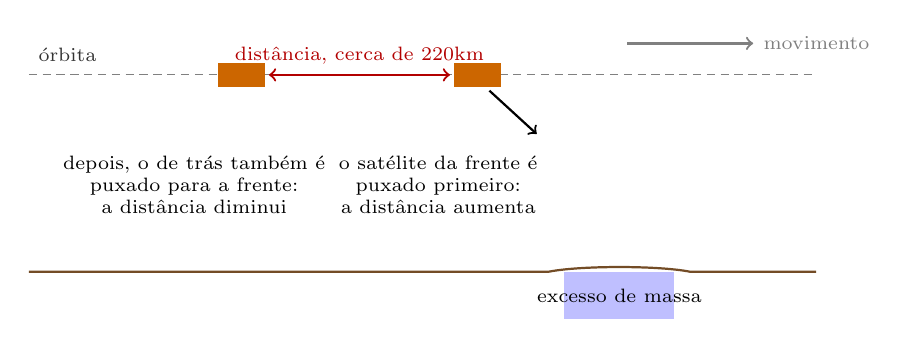
\begin{tikzpicture}[font=\small, x=1cm, y=1cm]
\draw[thick, brown!60!black] (-5,0) -- (1.6,0) .. controls (2.0,0.08) and (3.0,0.08) .. (3.4,0) -- (5,0);
\fill[blue!25] (1.8,0) rectangle (3.2,-0.6);
\node[font=\scriptsize] at (2.5,-0.3) {excesso de massa};
\draw[gray, densely dashed] (-5,2.5) -- (5,2.5);
\node[gray!40!black, font=\scriptsize, anchor=south west] at (-5,2.55) {órbita};
\fill[orange!80!black] (-2.6,2.35) rectangle (-2.0,2.65);
\fill[orange!80!black] (0.4,2.35) rectangle (1.0,2.65);
\draw[<->, red!70!black, thick] (-1.95,2.5) -- (0.35,2.5) node[midway, above, font=\scriptsize] {distância, cerca de \qty{220}{km}};
\draw[->, thick] (0.85,2.3) -- (1.45,1.75);
\draw[->, thick, gray] (2.6,2.9) -- (4.2,2.9) node[right, font=\scriptsize] {movimento};
\node[font=\scriptsize, anchor=north, align=center] at (0.2,1.6) {o satélite da frente é\\puxado primeiro:\\a distância aumenta};
\node[font=\scriptsize, anchor=north, align=center] at (-2.9,1.6) {depois, o de trás também é\\puxado para a frente:\\a distância diminui};
\end{tikzpicture}

\par\smallskip{\small O princípio do par de satélites (esquemático, fora de
escala). Ao se aproximar de um excesso de massa, o satélite da frente sente a atração dele
primeiro e é acelerado para a frente, de modo que a distância entre os dois aumenta; quando
o satélite de trás passa sobre a massa, a distância volta a diminuir. A taxa de variação da
distância, medida continuamente, é invertida para obter o campo de gravidade.}
\label{fig:b3:gravity-geodesy:grace}
\end{omfigure}

\begin{omfigure}
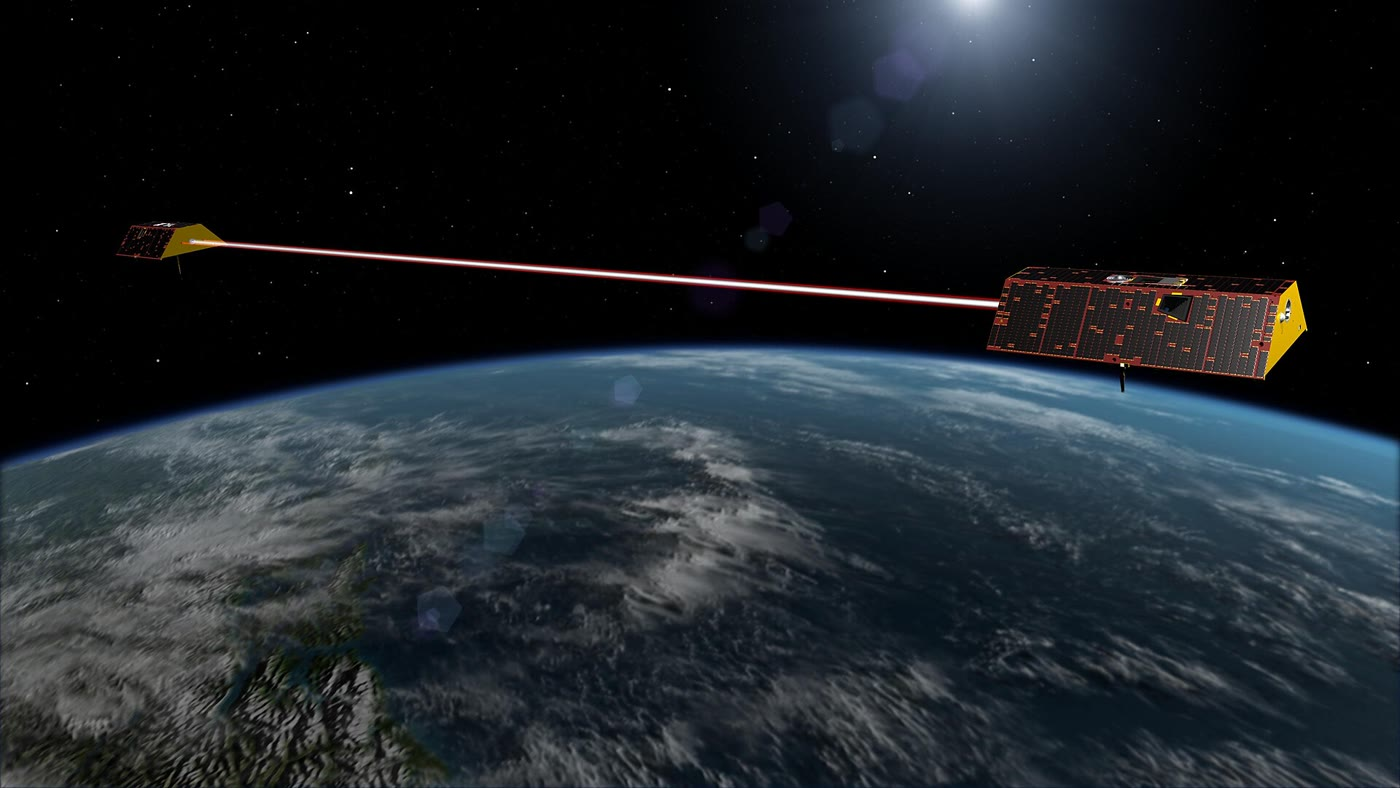
\includegraphics[width=0.66\linewidth]{images/book5/b3-grace-fo-concept.jpg}

\par\smallskip{\small Os dois satélites GRACE Follow-On, vista artística (a
distância entre eles está muito reduzida). O feixe vermelho representa o enlace
de medição de distância a laser. NASA/JPL-Caltech, domínio público.}
\label{fig:b3:gravity-geodesy:grace-photo}
\end{omfigure}

\begin{definition}[Altura equivalente de água]\label{def:b3:gravity-geodesy:ewh}
Uma variação do campo de gravidade que varia lentamente em distâncias muito maiores
que a espessura da camada onde a massa se deslocou pode ser representada por uma
variação da densidade superficial $\sigma$ (\unit{kg.m^{-2}}) em uma casca fina na
superfície da Terra. A \emph{altura equivalente de água}\index{altura equivalente de água}
é a espessura de água doce com a mesma densidade superficial:
\[
  h_w = \frac{\sigma}{\rho_w} .
\]
\end{definition}

Um metro de água sobre uma bacia de \qty{1e6}{km^2} corresponde a \qty{1e15}{kg}, ou
\qty{1000}{Gt}. O nível do mar é o outro lado da conta: \qty{360}{Gt} de gelo
acrescentados ao oceano elevam-no em cerca de um milímetro.
% ledger: data:b5-imbie
A \omterm{def:b3:gravity-geodesy:satgrav}{gravimetria por satélite}, a altimetria por satélite e o balanço entre a queda de neve e a
descarga de gelo medem, cada um, o balanço de massa dos mantos de gelo; reunidos, eles
fornecem a série abaixo.

\begin{omfigure}
\begin{tikzpicture}
\begin{axis}[omrecord, width=0.82\linewidth, height=0.5\linewidth,
  xmin=1992, xmax=2021, ymin=-5600, ymax=600,
  xlabel={ano}, ylabel={variação de massa acumulada (\unit{Gt})},
  xticklabel style={/pgf/number format/1000 sep={}},
  legend pos=south west, legend cell align=left, legend style={font=\scriptsize}]
\addplot[name path=gl, draw=none, forget plot] table[x=year, y=lo] {figdata/out/bachelor-3-ice_mass-greenland.dat};
\addplot[name path=gh, draw=none, forget plot] table[x=year, y=hi] {figdata/out/bachelor-3-ice_mass-greenland.dat};
\addplot[blue!25, forget plot] fill between[of=gl and gh];
\addplot[name path=al, draw=none, forget plot] table[x=year, y=lo] {figdata/out/bachelor-3-ice_mass-antarctica.dat};
\addplot[name path=ah, draw=none, forget plot] table[x=year, y=hi] {figdata/out/bachelor-3-ice_mass-antarctica.dat};
\addplot[red!20, forget plot] fill between[of=al and ah];
\addplot[blue!70!black, thick] table[x=year, y=cum] {figdata/out/bachelor-3-ice_mass-greenland.dat};
\addlegendentry{Groenlândia}
\addplot[red!70!black, thick] table[x=year, y=cum] {figdata/out/bachelor-3-ice_mass-antarctica.dat};
\addlegendentry{Antártida}
\draw[gray, densely dotted] (axis cs:2002.25,-5600) -- (axis cs:2002.25,600);
\draw[gray, densely dotted] (axis cs:2017.5,-5600) -- (axis cs:2017.5,600);
\node[font=\scriptsize, gray!40!black, anchor=north] at (axis cs:2009.9,550) {anos GRACE};
\end{axis}
\end{tikzpicture}

\par\smallskip{\small Variação de massa acumulada dos mantos de gelo da Groenlândia e da
Antártida desde 1992, com faixas de um desvio-padrão (estimativas reconciliadas do IMBIE 2021
a partir de altimetria, gravimetria e do método entrada--saída). Até o fim
de 2020, a Groenlândia havia perdido $\num{4890} \pm \qty{460}{Gt}$ e a Antártida
$\num{2670} \pm \qty{530}{Gt}$; ajustes em linha reta dão
\qty{-176}{Gt.yr^{-1}} e \qty{-91}{Gt.yr^{-1}} entre 1992 e 2020, e
\qty{-246}{Gt.yr^{-1}} e \qty{-127}{Gt.yr^{-1}} nos anos GRACE.}
\label{fig:b3:gravity-geodesy:ice-mass}
\end{omfigure}

Uma anomalia da gravidade medida na superfície é uma soma de harmônicos; na
altitude de um satélite, cada um é enfraquecido por um fator que depende de seu
comprimento de onda.

\begin{proposition}[Continuação para cima]\label{prop:b3:gravity-geodesy:upward}
Acima das massas que a causam, uma anomalia da gravidade que varia ao longo da superfície
como $\Delta g_0\cos kx$, com $k = 2\pi/\lambda$, vale, na altura $z$ (sua
\emph{continuação para cima}\index{continuação para cima}),
\[
  \Delta g(x, z) = \Delta g_0\,e^{-kz}\cos kx .
\]
\end{proposition}

\begin{proof}
Acima das massas, o potencial anômalo e, com ele, a anomalia satisfazem a
equação de Laplace $\partial_x^2\Delta g + \partial_z^2\Delta g = 0$. Separando as
variáveis, $\Delta g = Z(z)\cos kx$ com $Z'' = k^2Z$, cuja solução limitada quando
$z \to \infty$ é $Z = \Delta g_0e^{-kz}$.
\end{proof}

Na altitude de \qty{400}{km}, uma anomalia de \qty{1000}{km} de comprimento mantém \qty{8}{\percent}
de sua amplitude, e uma de \qty{100}{km} cerca de \num{1e-11} dela:
os satélites enxergam os comprimentos de onda longos, e os levantamentos na superfície, os curtos.

\section{Flexão da litosfera}

O volume do primeiro ano compensava uma carga localmente, cada coluna flutuando sobre si mesma.
Um vulcão sobre uma placa oceânica não é compensado apenas sob si mesmo: a
placa se curva sob ele numa largura de centenas de quilômetros, e o fundo do mar
ao redor do vulcão afunda num fosso, além do qual ele se eleva num arco baixo.

\begin{definition}[Flexão litosférica, rigidez flexural, espessura elástica efetiva]\label{def:b3:gravity-geodesy:flexure}
A \emph{flexão litosférica}\index{flexão litosférica} é a curvatura da
litosfera sob uma carga, modelada como a flexão de uma placa elástica fina
flutuando sobre um manto fluido. A resistência da placa à flexão é a sua
\emph{rigidez flexural}\index{rigidez flexural}
\[
  D = \frac{ET_e^3}{12(1 - \nu^2)},
\]
e a espessura $T_e$ da placa elástica uniforme que se curva como a litosfera real é a sua
\emph{espessura elástica efetiva}\index{espessura elástica efetiva}.
\end{definition}

\begin{theorem}[Flexão de uma placa fina]\label{thm:b3:gravity-geodesy:plate}
Uma placa elástica fina de rigidez $D$, curvada em uma direção por uma carga $q(x)$
por unidade de área, deslocada para baixo por $w(x)$ e flutuando sobre um manto de densidade
$\rho_m$, sendo a cavidade preenchida com material de densidade $\rho_i$, obedece à
\emph{equação da flexura}\index{equação da flexura}
\[
  D\frac{\mathrm d^4w}{\mathrm dx^4} + (\rho_m - \rho_i)g\,w = q(x) .
\]
\end{theorem}

\begin{proof}
Numa placa curvada, as fibras acima do plano médio são encurtadas e as abaixo
alongadas, em proporção à curvatura $w''$; integrando a tensão de flexão
ao longo da espessura obtém-se o momento fletor $M = -Dw''$, com a
rigidez da definição (a placa não pode se expandir lateralmente, daí o fator
$1 - \nu^2$; ver o volume do terceiro ano dos livros de física). Uma fatia $\mathrm dx$ da placa
carrega a força cortante $V$ em suas faces e o momento $M$. Equilíbrio vertical:
a carga $q\,\mathrm dx$ para baixo e o empuxo do manto deslocado
$(\rho_m - \rho_i)gw\,\mathrm dx$ para cima dão $\mathrm dV/\mathrm dx = -q +
(\rho_m - \rho_i)gw$. O equilíbrio de momentos dá $\mathrm dM/\mathrm dx = V$.
Então $-Dw'''' = M'' = V' = -q + (\rho_m - \rho_i)gw$.
\end{proof}

\begin{definition}[Parâmetro flexural, abaulamento periférico]\label{def:b3:gravity-geodesy:alpha}
O \emph{parâmetro flexural}\index{parâmetro flexural} de uma placa é o
comprimento
\[
  \alpha = \left(\frac{4D}{(\rho_m - \rho_i)g}\right)^{1/4},
\]
que fixa a escala horizontal de sua flexão. O \emph{abaulamento periférico}\index{abaulamento periférico}
é o arco baixo de flexão ascendente que a placa curvada levanta além do fosso ou da
bacia ao lado de sua carga.
\end{definition}

\begin{proposition}[Carga linear sobre uma placa contínua]\label{prop:b3:gravity-geodesy:line}
Uma carga linear $V_0$ por unidade de comprimento ao longo de $x = 0$ desloca a placa em
\[
  w(x) = w_0e^{-|x|/\alpha}\left(\cos\frac{|x|}{\alpha} + \sin\frac{|x|}{\alpha}\right),
  \qquad w_0 = \frac{V_0\alpha^3}{8D} .
\]
A deflexão se anula em $|x| = 3\pi\alpha/4$, a borda do fosso; a
crista do \omterm{def:b3:gravity-geodesy:alpha}{abaulamento periférico} está em $|x| = \pi\alpha$, com altura $w_0e^{-\pi} =
\num{0.0432}\,w_0$. O empuxo de toda a deflexão equilibra a carga:
$\int(\rho_m - \rho_i)gw\,\mathrm dx = V_0$.
\end{proposition}

\begin{proof}
Para $x > 0$ a equação é $w'''' + 4w/\alpha^4 = 0$; as raízes de
$r^4 = -4/\alpha^4$ são $(\pm1 \pm i)/\alpha$, e as soluções que se anulam ao longe
são $e^{-x/\alpha}(A\cos(x/\alpha) + B\sin(x/\alpha))$. A simetria impõe
$w'(0) = 0$, o que dá $A = B = w_0$. Integrando o balanço vertical através
da carga, a força cortante $V = -Dw'''$ sofre um salto de $-V_0$; por simetria
$w'''(0^-) = -w'''(0^+)$, e $w'''(0^+) = 4w_0/\alpha^3$, logo $8Dw_0/\alpha^3 =
V_0$. A deflexão se anula onde $\tan(x/\alpha) =
-1$, pela primeira vez em $x = 3\pi\alpha/4$; sua derivada,
$-(2w_0/\alpha)e^{-x/\alpha}\sin(x/\alpha)$, se anula em seguida em $x = \pi\alpha$.
Por fim, $\int_0^\infty e^{-u}(\cos u + \sin u)\,\mathrm du = 1$, logo
$\int w\,\mathrm dx = 2w_0\alpha = V_0\alpha^4/(4D) = V_0/((\rho_m - \rho_i)g)$.
\end{proof}

\begin{proposition}[Placa quebrada]\label{prop:b3:gravity-geodesy:broken}
Uma placa quebrada em $x = 0$ e empurrada para baixo em sua extremidade livre, como numa fossa
oceânica profunda, desloca-se segundo $w = w_0e^{-x/\alpha}\cos(x/\alpha)$ para $x \ge 0$: a
deflexão se anula em $x = \pi\alpha/2$, e a crista do \omterm{def:b3:gravity-geodesy:alpha}{abaulamento periférico}, a
elevação externa, está em $x = 3\pi\alpha/4$, com altura $w_0e^{-3\pi/4}/\sqrt2 =
\num{0.067}\,w_0$.
\end{proposition}

\begin{proof}
As mesmas soluções decrescentes, agora com a extremidade livre sem momento,
$w''(0) = 0$, o que dá $B = 0$. O zero está em $\cos(x/\alpha) = 0$; a
derivada $-(w_0/\alpha)e^{-x/\alpha}(\cos + \sin)(x/\alpha)$ se anula em
$x = 3\pi\alpha/4$, onde $w = w_0e^{-3\pi/4}\cos(3\pi/4)$.
\end{proof}

Assim, as distâncias são a chave para a resistência da placa: meça onde termina o fosso
ou onde o abaulamento atinge a crista, e $\alpha$ segue, depois $D$, depois $T_e$.
Como $T_e$ entra como $\alpha^{4/3}$, uma boa estimativa de uma distância dá uma boa
estimativa da espessura.

\begin{omfigure}
\begin{tikzpicture}
\begin{groupplot}[group style={group size=1 by 2, vertical sep=1.5cm},
  width=0.82\linewidth, height=0.36\linewidth, xmin=-400, xmax=400,
  tick label style={font=\scriptsize}, label style={font=\small}, title style={font=\small}]
\nextgroupplot[title={(a) carga linear: a cordilheira de Oru sobre placas de três espessuras},
  ylabel={deflexão (\unit{m})}, ymin=-3000, ymax=700, y filter/.expression={-y},
  legend pos=south east, legend cell align=left, legend style={font=\scriptsize}]
\addplot[red!70!black, thick] table[x=x, y=w10] {figdata/out/bachelor-3-flexure-profiles.dat};
\addlegendentry{$T_e = \qty{10}{km}$}
\addplot[blue!70!black, thick] table[x=x, y=w25] {figdata/out/bachelor-3-flexure-profiles.dat};
\addlegendentry{$T_e = \qty{25}{km}$}
\addplot[green!45!black, thick] table[x=x, y=w40] {figdata/out/bachelor-3-flexure-profiles.dat};
\addlegendentry{$T_e = \qty{40}{km}$}
\draw[gray] (axis cs:-400,0) -- (axis cs:400,0);
\draw[->, blue!70!black] (axis cs:222,330) -- (axis cs:222,90);
\node[font=\scriptsize, blue!70!black, anchor=south] at (axis cs:222,330) {abaulamento periférico, $\pi\alpha$};
\nextgroupplot[title={(b) placa quebrada numa fossa, $T_e = \qty{25}{km}$},
  xlabel={distância da carga ou da fossa (\unit{km})},
  ylabel={deflexão (\unit{m})}, xmin=0, xmax=400, ymin=-1100, ymax=280,
  y filter/.expression={-y}]
\addplot[blue!70!black, thick] table[x=x, y=w] {figdata/out/bachelor-3-flexure-broken.dat};
\draw[gray] (axis cs:0,0) -- (axis cs:400,0);
\draw[->] (axis cs:166.5,200) -- (axis cs:166.5,80);
\node[font=\scriptsize, anchor=west] at (axis cs:170,200) {elevação externa, $3\pi\alpha/4$};
\end{groupplot}
\end{tikzpicture}

\par\smallskip{\small Flexão de uma placa elástica (calculada;
$E = \qty{100}{GPa}$, $\nu = 0.25$, manto \qty{3300}{kg.m^{-3}}, água no
fosso; escala vertical muito exagerada). (a) Sob a carga de uma crista
vulcânica (\qty{4.17e12}{N.m^{-1}}), uma placa fina afunda profunda e estreitamente, uma
placa espessa, rasa e largamente; o \omterm{def:b3:gravity-geodesy:alpha}{abaulamento periférico} se desloca de \qty{112}{km} para
\qty{316}{km}. (b) Uma placa rompida numa fossa e empurrada para baixo em \qty{1}{km}:
a elevação externa tem \qty{67}{m} de altura, a \qty{167}{km} da fossa.}
\label{fig:b3:gravity-geodesy:flexure}
\end{omfigure}

\begin{definition}[Compensação isostática regional]\label{def:b3:gravity-geodesy:regional}
A \emph{compensação isostática regional}\index{compensação isostática regional}
é o suporte de uma carga pelo empuxo de uma deflexão distribuída por uma região
mais larga que a carga, por meio da resistência à flexão da litosfera; na
compensação de Airy ou de Pratt, em contraste, cada coluna é compensada sob si mesma.
\end{definition}

A compensação local e a regional equilibram a mesma massa total, mas a distribuem
de modo diferente: sob uma carga estreita numa placa rígida, a raiz é rasa e larga,
e a anomalia da gravidade sobre a carga é fortemente positiva, ladeada por
anomalias negativas sobre o fosso. Ao redor das ilhas da Cadeia Havaiana, perfis gravimétricos e
sísmicos dão \omterm{def:b3:gravity-geodesy:flexure}{espessuras elásticas efetivas} de 17 a \qty{37}{km}, e
de 10 a \qty{20}{km} ao longo dos montes submarinos mais antigos da cadeia Imperador, uma diferença
esperada a partir das idades dos vulcões e da placa que carregaram; os valores
acompanham a profundidade de uma isoterma próxima de
\qty{350}{\degreeCelsius} na placa oceânica em resfriamento.
% ledger: watts25:te
A mesma flexão, sob o peso de um cinturão de montanhas, abre as bacias de
antepaís do volume do segundo ano, no capítulo sobre o orógeno alpino.

\begin{omfigure}
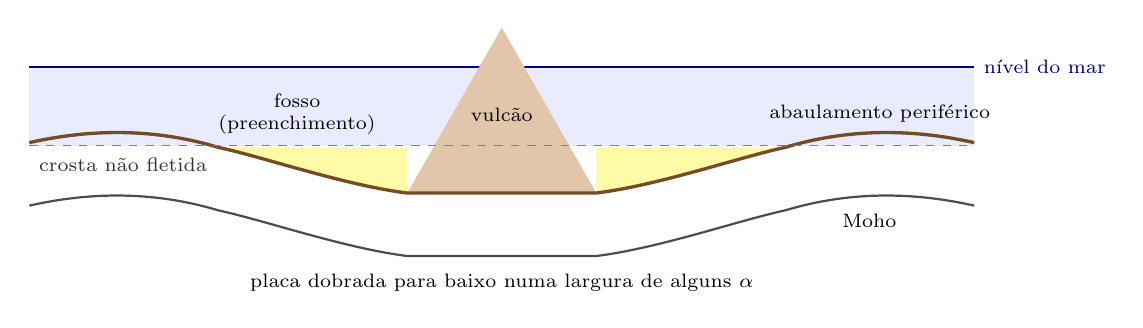
\begin{tikzpicture}[font=\scriptsize, x=1cm, y=1cm]
\fill[blue!8] (-6,0) rectangle (6,-1.0);
\draw[blue!50!black] (-6,0) -- (6,0) node[right] {nível do mar};
% volcano
\fill[brown!45] (-1.2,-1.6) -- (0,0.5) -- (1.2,-1.6) -- cycle;
% moat infill
\fill[yellow!35] (-1.2,-1.6) .. controls (-2.0,-1.5) and (-3.0,-1.15) .. (-3.6,-1.02) -- (-1.2,-1.02) -- cycle;
\fill[yellow!35] (1.2,-1.6) .. controls (2.0,-1.5) and (3.0,-1.15) .. (3.6,-1.02) -- (1.2,-1.02) -- cycle;
% flexed seafloor (top of crust)
\draw[very thick, brown!60!black] (-6,-0.96) .. controls (-5.2,-0.78) and (-4.4,-0.78) .. (-3.6,-1.02)
  .. controls (-3.0,-1.15) and (-2.0,-1.5) .. (-1.2,-1.6) -- (1.2,-1.6)
  .. controls (2.0,-1.5) and (3.0,-1.15) .. (3.6,-1.02) .. controls (4.4,-0.78) and (5.2,-0.78) .. (6,-0.96);
% Moho, parallel
\draw[thick, gray!60!black] (-6,-1.76) .. controls (-5.2,-1.58) and (-4.4,-1.58) .. (-3.6,-1.82)
  .. controls (-3.0,-1.95) and (-2.0,-2.3) .. (-1.2,-2.4) -- (1.2,-2.4)
  .. controls (2.0,-2.3) and (3.0,-1.95) .. (3.6,-1.82) .. controls (4.4,-1.58) and (5.2,-1.58) .. (6,-1.76);
\node[anchor=west] at (4.2,-1.95) {Moho};
\draw[dashed, gray] (-6,-1.0) -- (6,-1.0);
\node[anchor=north west, gray!40!black] at (-6,-1.03) {crosta não fletida};
\node[anchor=south, align=center] at (-2.6,-0.98) {fosso\\(preenchimento)};
\node[anchor=south] at (4.8,-0.82) {abaulamento periférico};
\node at (0,-0.6) {vulcão};
\node[anchor=north] at (0,-2.5) {placa dobrada para baixo numa largura de alguns $\alpha$};
\end{tikzpicture}

\par\smallskip{\small Uma ilha vulcânica sobre uma placa oceânica (seção
transversal esquemática, escala vertical exagerada). A placa se curva sob o
vulcão; a depressão ao redor dele, o fosso, se preenche de detritos vulcânicos
e sedimentos, e, além dele, a placa se eleva num \omterm{def:b3:gravity-geodesy:alpha}{abaulamento periférico} baixo.}
\label{fig:b3:gravity-geodesy:moat}
\end{omfigure}

\begin{inthefield}[Um levantamento gravimétrico relativo]
\begin{minipage}[t]{0.55\linewidth}\vspace{0pt}
Um gravímetro absoluto solta um espelho de canto numa câmara de vácuo, de novo
e de novo, e cronometra a queda com um interferômetro a laser e um relógio atômico;
ele fornece a gravidade em uma estação, mas é pesado e lento para montar. O levantamento
em si é feito com um gravímetro relativo, uma pequena balança de mola que mede
diferenças de gravidade. O geofísico o nivela sobre uma placa-base em cada
estação de uma linha, faz a leitura, anota a hora e a altura, e segue adiante; a cada
poucas horas, a malha retorna a uma estação-base, de modo que a deriva lenta da
mola e as marés da Terra sólida possam ser medidas e removidas. Um receptor de satélite
sobre um polo próximo fornece a posição e a altura, pois a gravidade
muda cerca de \qty{0.3}{\milli\gal} para cada metro de altura.
\end{minipage}\hfill
\begin{minipage}[t]{0.42\linewidth}\vspace{0pt}
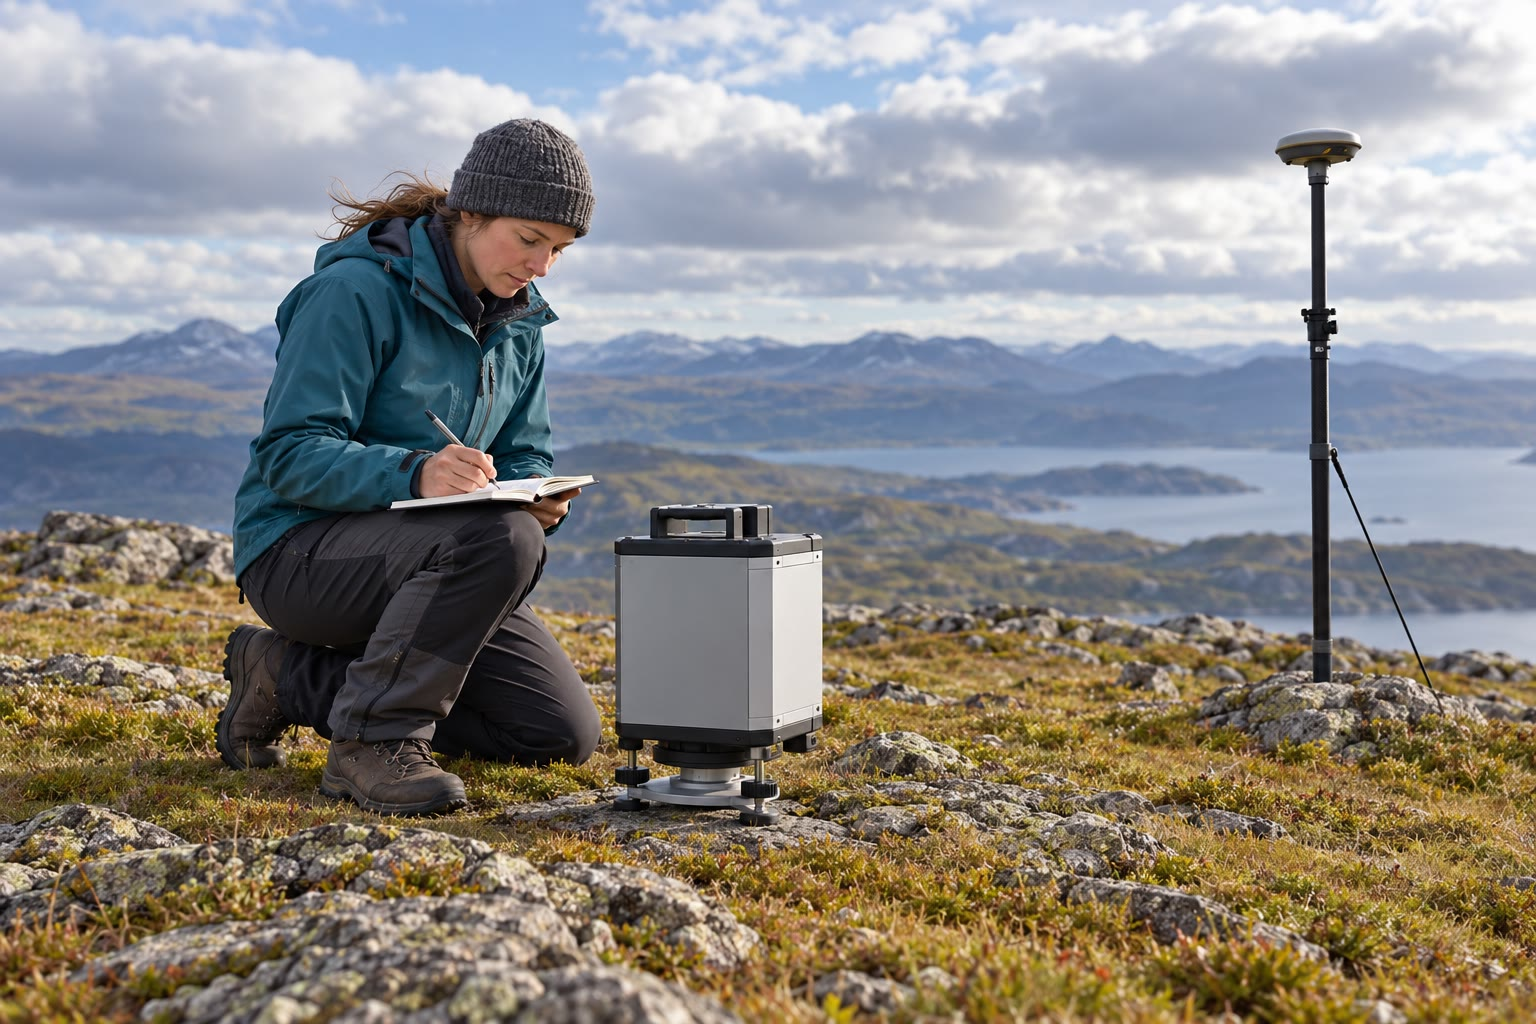
\includegraphics[width=\linewidth]{images/book5/ai/b3-gravimeter.jpg}

{\scriptsize Um gravímetro de campo sobre sua base de nivelamento, com uma antena
de satélite ao fundo (ilustração gerada por IA).}
\end{minipage}
\end{inthefield}

\section{Exercícios}

\begin{exercise}[$\star$]\label{exo:b3:gravity-geodesy:1}
A partir dos valores do Sistema Geodésico de Referência 1980 $a = \qty{6378137}{m}$ e
$f = \num{0.00335281068}$, calcule o semieixo menor $b$ e $a - b$. Com
$J_2 = \num{1.08263e-3}$ e $m = \num{0.00344979}$, calcule o achatamento que
a relação de Clairaut prevê, e compare.
\end{exercise}

\begin{exercise}[$\star$]\label{exo:b3:gravity-geodesy:2}
Em um ano seco, uma bacia fluvial de \qty{5.0e5}{km^2} perde \qty{60}{Gt} de
água. Calcule a variação da \omterm{def:b3:gravity-geodesy:ewh}{altura equivalente de água}. Quanto subiria o
nível do mar com a mesma massa, tomando \qty{360}{Gt} por milímetro?
\end{exercise}

\begin{exercise}[$\star$]\label{exo:b3:gravity-geodesy:3}
Com a série $\gamma = 9.780327(1 + 0.0053024\sin^2\varphi -
0.0000058\sin^22\varphi)$ \unit{m.s^{-2}}, calcule a gravidade normal no
equador, em \ang{45} e nos polos. Expresse a diferença entre o polo
e o equador em miligals.
\end{exercise}

\begin{exercise}[$\star$]\label{exo:b3:gravity-geodesy:4}
Calcule a \omterm{def:b3:gravity-geodesy:flexure}{rigidez flexural} e o \omterm{def:b3:gravity-geodesy:alpha}{parâmetro flexural} de placas oceânicas com
$T_e = \qty{10}{km}$ e $T_e = \qty{30}{km}$ ($E = \qty{100}{GPa}$,
$\nu = 0.25$, $\rho_m - \rho_w = \qty{2270}{kg.m^{-3}}$, $g =
\qty{9.81}{m.s^{-2}}$). Onde estão a borda do fosso e o \omterm{def:b3:gravity-geodesy:alpha}{abaulamento periférico} sob uma
carga linear?
\end{exercise}

\begin{exercise}[$\star\star$]\label{exo:b3:gravity-geodesy:5}
(a) Para uma altura do geoide de $+\qty{50}{m}$, calcule o potencial perturbador ali,
tomando $\gamma = \qty{9.80}{m.s^{-2}}$. (b) Sobre \qty{100}{km}, o geoide sobe
em \qty{10}{m}. Por que ângulo a linha de prumo ali difere da normal ao
elipsoide? Expresse-o em segundos de arco.
\end{exercise}

\begin{exercise}[$\star\star$]\label{exo:b3:gravity-geodesy:6}
A partir de $J_2 = \num{1.08263e-3}$ e do fator de momento de inércia
$C/(Ma^2) = \num{0.3308}$, calcule a elipticidade dinâmica $H = (C - A)/C$ e
$1/H$. Qual dos dois números alteraria uma Terra homogênea com o mesmo $J_2$?
\end{exercise}

\begin{exercise}[$\star\star$]\label{exo:b3:gravity-geodesy:7}
Um satélite percorre uma órbita circular a \qty{500}{km} acima do raio equatorial
($a = \qty{6378.137}{km}$, $GM = \qty{3.986005e14}{m^3.s^{-2}}$), com inclinação de
\ang{89}. Calcule seu período e a taxa de precessão nodal em graus por dia.
Por que as missões de gravimetria escolhem órbitas quase polares?
\end{exercise}

\begin{exercise}[$\star\star$]\label{exo:b3:gravity-geodesy:8}
Duas anomalias de \qty{10}{\milli\gal} na superfície têm comprimentos de onda de
\qty{100}{km} e \qty{1000}{km}. Calcule suas amplitudes a
\qty{500}{km} de altitude.
\end{exercise}

\begin{exercise}[$\star\star$]\label{exo:b3:gravity-geodesy:9}
No lado oceânico de uma fossa, a crista do abaulamento externo fica a \qty{120}{km} do
eixo da fossa. Adotando o modelo de placa quebrada com água sobre a placa, calcule
$\alpha$, $D$ e $T_e$, e a distância em que a placa cruza seu nível não
fletido.
\end{exercise}

\begin{exercise}[$\star\star\star$]\label{exo:b3:gravity-geodesy:10}
(a) Verifique que $w = w_0e^{-u}(\cos u + \sin u)$, $u = x/\alpha$, satisfaz
$Dw'''' + (\rho_m - \rho_i)gw = 0$ para $x > 0$, com $\alpha$ conforme definido.
(b) Mostre que o momento fletor $-Dw''$ é máximo sob a carga e muda
de sinal em $x = \pi\alpha/4$. (c) Onde a placa tem maior probabilidade de fraturar
na sua superfície superior, e por quê?
\end{exercise}

\begin{exercise}[$\star\star\star$]\label{exo:b3:gravity-geodesy:11}
Com $m = \num{0.00344979}$ e $C/(Ma^2) = \num{0.3308}$, inverta a
relação de Darwin--Radau para o achatamento hidrostático. Compare com
$f = \num{0.00335281}$: calcule a diferença e o excesso de altura do
equador acima da forma hidrostática. O que isso diz sobre o manto?
\end{exercise}

\begin{exercise}[$\star\star\star$]\label{exo:b3:gravity-geodesy:12}
Um satélite em órbita circular a \qty{700}{km} de altura deve manter a mesma
orientação em relação ao Sol durante todo o ano: seu nodo deve avançar \ang{360} em
um ano trópico de \num{365.242}~dias. Calcule a inclinação necessária.
\end{exercise}

\section{Problema: O fosso em torno da cordilheira Oru}

\begin{problem}[{Problema de fim de semana --- a figura da Terra, uma carga vulcânica,
seu fosso flexural e o que os satélites veem dele}]
\label{pb:b3:gravity-geodesy:1}
% values: calc/ch03.py; GRS80 (geod5:grs80-*), earth:MoI; flexure.py
Oru é uma cordilheira vulcânica fictícia em um oceano: uma cadeia retilínea de vulcões coalescidos
com \qty{400}{km} de comprimento, construída sobre litosfera oceânica antiga. Sua
seção transversal é tomada como um triângulo com \qty{80}{km} de largura na base e
\qty{6}{km} de altura, de densidade \qty{2800}{kg.m^{-3}}, assentado sobre um fundo marinho
\qty{5}{km} de profundidade. Manto \qty{3300}{kg.m^{-3}}, água do mar
\qty{1030}{kg.m^{-3}}, $E = \qty{100}{GPa}$, $\nu = 0.25$, $g =
\qty{9.81}{m.s^{-2}}$, $G = \qty{6.674e-11}{m^3.kg^{-1}.s^{-2}}$.

\medskip
\noindent\textbf{Parte I --- A figura da Terra.} Use o Sistema Geodésico de Referência
de 1980: $a = \qty{6378137}{m}$, $b = \qty{6356752.3}{m}$,
$GM = \qty{3.986005e14}{m^3.s^{-2}}$, $J_2 = \num{1.08263e-3}$,
$\omega = \qty{7.292115e-5}{rad.s^{-1}}$, $f = \num{0.00335281}$; e
$C/(Ma^2) = \num{0.3308}$.
\begin{enumerate}
  \item Calcule $m = \omega^2a^2b/(GM)$.
  \item Calcule o achatamento dado pela relação de Clairaut a partir de $J_2$ e
        $m$, e seu inverso.
  \item Calcule o achatamento hidrostático a partir da relação de Darwin--Radau, e
        seu inverso.
  \item Compare ambos com o achatamento observado. Em quantos metros o
        equador se eleva acima da figura hidrostática?
  \item Calcule a elipticidade dinâmica $H = (C - A)/C$.
\end{enumerate}

\noindent\textbf{Parte II --- A carga.}
\begin{enumerate}[resume]
  \item Calcule a área da seção transversal da cordilheira.
  \item Calcule a carga linear $V_0$, tomando a cordilheira inteira como submersa, de modo
        que ela pese $(\rho_v - \rho_w)g$ por unidade de volume.
  \item Se a cordilheira fosse compensada localmente, à maneira de Airy, por uma raiz de
        rocha própria no manto, qual seria a profundidade da raiz sob a
        crista?
  \item Sob compensação local, a raiz terminaria no pé da cordilheira,
        a \qty{40}{km} de seu eixo. A batimetria mostra um fosso até
        \qty{165}{km}. O que isso indica?
\end{enumerate}

\noindent\textbf{Parte III --- O fosso flexural.} O fosso está preenchido com água
($\rho_i = \rho_w$). Um perfil sísmico atravessando a cordilheira encontra o topo da
crosta oceânica de volta à sua profundidade regional a \qty{165}{km} do eixo, e a
crista do \omterm{def:b3:gravity-geodesy:alpha}{abaulamento periférico} a \qty{220}{km} do eixo.
\begin{enumerate}[resume]
  \item Calcule o \omterm{def:b3:gravity-geodesy:alpha}{parâmetro flexural} a partir da borda do fosso.
  \item Calcule-o novamente a partir do \omterm{def:b3:gravity-geodesy:alpha}{abaulamento periférico}. Os dois valores são consistentes?
  \item Tomando $\alpha = \qty{70.0}{km}$, calcule a \omterm{def:b3:gravity-geodesy:flexure}{rigidez flexural}.
  \item Calcule a \omterm{def:b3:gravity-geodesy:flexure}{espessura elástica efetiva}.
  \item Tomando $V_0 = \qty{4.17e12}{N.m^{-1}}$ e $D$ arredondado para três
        algarismos significativos, calcule a deflexão sob o eixo.
  \item Calcule a altura do \omterm{def:b3:gravity-geodesy:alpha}{abaulamento periférico}.
  \item Verifique que o empuxo de toda a deflexão, $2w_0\alpha(\rho_m -
        \rho_w)g$, equilibra $V_0$.
  \item Compare $T_e$ com os valores encontrados ao longo da cordilheira havaiana, de 17 a
        \qty{37}{km}. Compare a deflexão sob o eixo com a
        raiz de Airy da pergunta 8.
\end{enumerate}

\noindent\textbf{Parte IV --- Gravidade sobre o fosso.} Considere um harmônico da
flexura, de comprimento de onda $2\pi\alpha$ e amplitude $W = \qty{500}{m}$, deformando
tanto o fundo marinho (crosta de \qty{2900}{kg.m^{-3}} sob a água, a \qty{5}{km} abaixo
do nível do mar) e o Moho (manto sob a crosta, a \qty{12}{km} abaixo do nível do mar). Uma
camada delgada de densidade superficial $\sigma$ produz a anomalia $2\pi G\sigma$
logo acima dela.
\begin{enumerate}[resume]
  \item Calcule o comprimento de onda e o número de onda $k$ do harmônico.
  \item Calcule a amplitude da anomalia ao nível do mar devida ao fundo marinho
        deformado, continuado para cima a partir de \qty{5}{km} de profundidade.
  \item Calcule a do Moho deformado, e o total.
  \item Calcule o total na altitude de um satélite, a \qty{400}{km} acima do nível do
        mar.
  \item Por qual fator um harmônico de comprimento de onda \qty{80}{km}, a largura da
        cordilheira, é atenuado nessa altitude? O que o satélite consegue resolver?
  \item A qual grau de harmônico esférico $n \approx 2\pi R/\lambda$ corresponde o
        harmônico da pergunta 18 ($R = \qty{6371}{km}$)?
  \item Dê a \omterm{def:b3:gravity-geodesy:flexure}{espessura elástica efetiva} da placa sob a
        cordilheira Oru.
\end{enumerate}
\end{problem}
